% Sumber: docs/ARCHITECTURE.md, docs/EXPERIMENT.md (EXP-005/006/007), docs/EXP-007_ARCFACE_EVALUATION.md,
% docs/ARCFACE_EXPERIMENT_DESIGN.md, docs/R7_5_CLASS_DECISION.md, docs/reports/PAPUAN_V2_*.md,
% src/{frame_extractor,face_detector,emotion_classifier,landmark_analyzer}.py,
% tools/{extract_arcface_embeddings,train_arcface_classifier}.py, RESEARCH_DECISIONS.md,
% docs/EXP-010_FAIRNESS_135.md, docs/EXP-011_CLAHE_FAIRNESS_135.md,
% tools/{analyze_fairness_135,analyze_clahe_fairness_135}.py, research-audit/D8_SKIN_TONE_DISCREPANCY_INVESTIGATION.md.
\chapter{Metodologi Penelitian}
\label{chap:methodology}

\section{Rancangan Penelitian}

Rancangan penelitian utama adalah evaluasi keadilan (\textit{fairness}): mengukur kesenjangan kinerja antara kelompok kecerahan Gelap dan Gelap-Sedang untuk satu model FER terlatih (HSEmotion), lalu memeriksa apakah satu varian praproses (CLAHE) atau satu klasifier alternatif (ArcFace + Regresi Logistik) mengubah kesenjangan tersebut, pada dataset yang disusun proyek ini dari satu film sumber (\S\ref{sec:dataset-overview}). Prediksi dihasilkan oleh EXP-005 sampai EXP-007; kesenjangan antar-kelompok beserta selang kepercayaannya dihitung oleh EXP-010 dan EXP-011 sebagai analisis ulang atas prediksi yang sudah tersimpan (\S\ref{sec:fairness-methods}). Ini bukan eksperimen terkontrol dalam arti acak (\textit{randomized}): hanya ada satu sampel, bukan kelompok perlakuan dan kelompok kontrol yang diambil dari populasi yang sama, sehingga lebih tepat disebut studi kasus yang terinstrumentasi dengan baik: model tetap, varian praproses tetap, masing-masing diterapkan satu kali pada sampel yang tetap, dengan prediksi yang dihasilkan dibandingkan terhadap kebenaran lapangan manual di bawah uji statistik eksplisit di mana ukuran sampel memungkinkan. Satu jalur kedua yang berjalan paralel, yaitu uji coba anotasi titik-fitur wajah Papuan V2 (\S\ref{sec:methodology-landmarks}), adalah pekerjaan infrastruktur penyusunan dataset dan anotasi, yang sudah ditegaskan penulis sebagai pendukung, bukan utama (\texttt{RESEARCH\_DECISIONS.md}, Keputusan 2); jalur ini dijelaskan di sini sebatas tahap yang benar-benar sudah dicapai.

\begin{figure}[htbp]
\centering
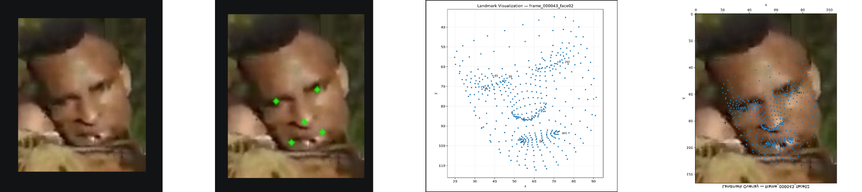
\includegraphics[width=0.85\textwidth]{figures/ringkasan-pipeline-wajah}
\caption[Ringkasan alur satu potongan wajah melalui pipeline]{Ringkasan alur satu potongan wajah melalui \textit{pipeline}: potongan wajah hasil deteksi, titik fitur geometris (empat titik hijau) yang dipakai untuk fitur jarak alis/bibir/mulut, visualisasi titik-fitur \textit{mesh} 468-titik MediaPipe, dan hasil tumpang-susun \textit{mesh} tersebut pada potongan wajah yang sama.}
\label{fig:ringkasan-pipeline}
\end{figure}

Gambar~\ref{fig:ringkasan-pipeline} memberi gambaran sekilas tentang apa yang dimaksud ``potongan wajah'' dan ``titik-fitur'' di seluruh bab ini, sebelum rinciannya dijelaskan per komponen pada \S\ref{sec:dataset-overview} dan \S\ref{sec:methodology-landmarks}.

\section{Dataset Lama dan Dua Populasi Evaluasi}
\label{sec:dataset-overview}

Seluruh eksperimen FER (EXP-005 sampai EXP-008, serta analisis ulang EXP-010 dan EXP-011) memakai potongan dari satu video sumber: film dokumenter pesta babi masyarakat Papua, resolusi 1920$\times$1080, berdurasi sekitar 96 menit, 144.084 \textit{frame} pada 25 fps.

\begin{figure}[htbp]
\centering
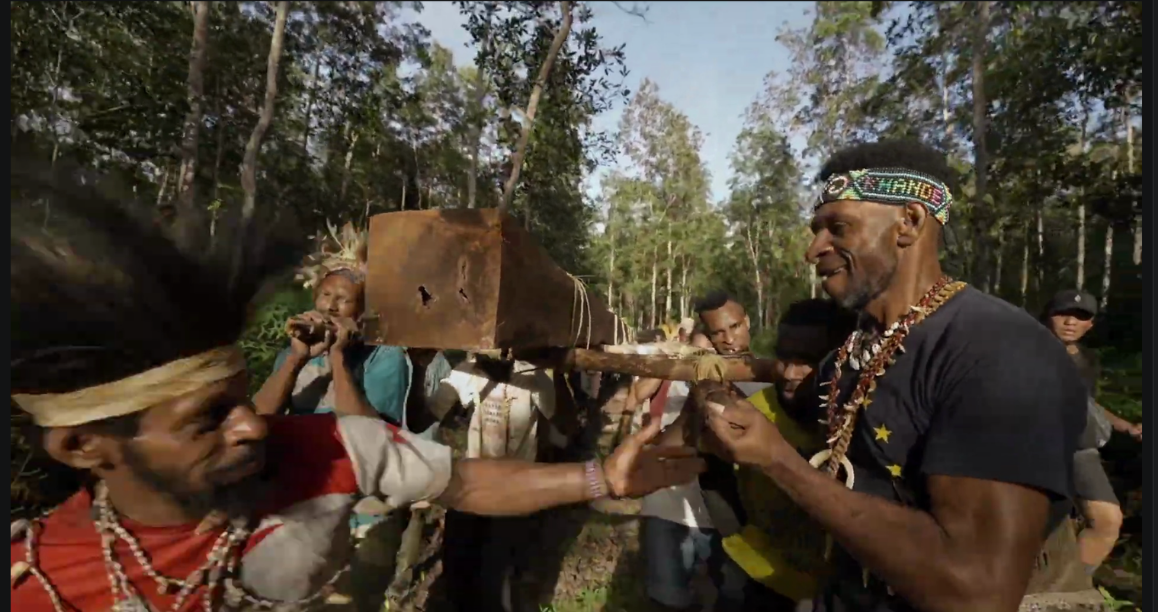
\includegraphics[width=0.7\textwidth]{figures/contoh-frame-sumber}
\caption[Contoh satu frame dari film sumber]{Contoh satu \textit{frame} dari film sumber, sebelum deteksi wajah dijalankan.}
\label{fig:contoh-frame-sumber}
\end{figure}

Gambar~\ref{fig:contoh-frame-sumber} menunjukkan satu \textit{frame} mentah seperti ini, sebelum tahap deteksi wajah (\S\ref{sec:arcface-config} di bawah, dan \S\ref{sec:clahe-config}) dijalankan terhadapnya. Satu kali jalan \textit{pipeline} berskala uji-coba (\textit{debug-scale}) terhadap 100 \textit{frame} yang diambil sampelnya menghasilkan 227 potongan wajah terdeteksi melalui paket \texttt{buffalo\_l} milik InsightFace (pendeteksi SCRFD, bantalan kotak pembatas 20\%). Setiap satu dari 227 potongan itu diperiksa secara manual oleh satu orang anotator dan diberi salah satu dari tujuh label: Netral (80), Ambigu (83), Senang (34), Sedih (12), Jijik (2), Takut (7), Terkejut (8), Marah (1). Tidak ada anotator kedua yang memeriksa label-label ini, dan proyek ini tidak memiliki statistik kesepakatan antar-anotator untuknya. Batasan ini berlaku untuk setiap hasil dalam bab ini dan bab berikutnya, dinyatakan sekali di sini.

Untuk setiap potongan, kelompok warna kulit dihitung langsung dari data piksel: kombinasi berbobot dari rata-rata, median, dan rata-rata wilayah tengah kanal-L ruang warna LAB (\texttt{src/landmark\_analyzer.py}, fungsi \texttt{\_compute\_skin\_tone}), diberi ambang batas menjadi beberapa kelompok (Gelap di bawah 100, Gelap-Sedang di bawah 150, dan seterusnya). Ini adalah statistik kecerahan, bukan pengukuran demografis, dan disebut sebagai ``proksi warna kulit'' di seluruh tesis ini agar perbedaan ini tetap terlihat dalam teks, tidak hanya di catatan kaki. Pada sampel 227 potongan, fungsi ini menghasilkan 159 potongan Gelap, 65 Gelap-Sedang, dan 3 Gelap-Terang, bukan populasi yang nyaris seragam seperti yang diasumsikan oleh deskripsi internal dataset ini sebelumnya. (Pembagian kira-kira 59\%/41\% yang pernah dilaporkan berasal dari 85 potongan yang memiliki fitur titik-fitur wajah, bukan dari seluruh 227 potongan; \texttt{research-audit/D8\_SKIN\_TONE\_DISCREPANCY\_INVESTIGATION.md}.)

\textbf{Dua populasi dipakai dalam eksperimen-eksperimen ini, dan keduanya tidak bisa dipertukarkan begitu saja.} EXP-005 dan EXP-006 mengevaluasi HSEmotion terhadap seluruh sampel 227 potongan dalam pelabelan tujuh-kelas aslinya. EXP-007 mengevaluasi baik HSEmotion maupun klasifier berbasis ArcFace pada subset turunan berjumlah 135 potongan, dibatasi menjadi lima kelas (Takut, Senang, Netral, Sedih, Terkejut). Subset 135 potongan inilah populasi utama untuk ketiga RQ: EXP-010 (RQ1, RQ3) dan EXP-011 (RQ2) menghitung kesenjangan antar-kelompok pada subset ini, sedangkan hasil pada 227 potongan dipakai hanya sebagai bukti pendukung. Subset 135 potongan ini bukan sampel yang dikumpulkan terpisah; subset ini adalah populasi 227 potongan yang disaring melalui tiga langkah pengecualian berturut-turut, masing-masing dengan penyebab yang konkret dan terdokumentasi:

\begin{enumerate}
  \item 83 potongan berlabel \texttt{Ambigu} dibuang, karena ``Ambigu'' bukan kelas ekspresi target dan klasifier tidak punya cara yang berprinsip untuk dinilai terhadapnya. $227 - 83 = 144$.
  \item 1 potongan \texttt{Marah} dan 2 potongan \texttt{Jijik} dibuang sebagai pengecualian kelas jarang, karena keduanya tidak punya cukup kejadian untuk mendukung metrik per-kelas yang dapat diandalkan pada ukuran sampel ini. $144 - 3 = 141$.
  \item 6 potongan lagi hilang akibat kegagalan deteksi ulang ArcFace: \textit{pipeline} ArcFace menjalankan ulang deteksi wajah pada setiap potongan yang sudah ada sebelum mengekstraksi \textit{embedding}-nya (\S\ref{sec:arcface-config}), dan 6 dari 141 potongan yang memenuhi syarat label gagal pada langkah deteksi ulang ini sehingga dikecualikan. $141 - 6 = 135$.
\end{enumerate}

Rangkaian ini dikuatkan oleh dua dokumen proyek yang independen, yaitu hitungan titik-periksa laporan evaluasi R6/R7 (227 $\to$ 178 berhasil dideteksi ulang $\to$ 144 memenuhi syarat label $\to$ 135 akhir) dan urutan penyaringan yang ditetapkan dalam dokumen rancangan eksperimen, dan penggabungan datanya sendiri berbasis identitas (dicocokkan berdasarkan nama berkas potongan wajah, diverifikasi secara terprogram), bukan berdasarkan posisi baris. Satu bukti konkret yang menguatkan hal ini: 18 kesalahan klasifikasi Netral-menjadi-Marah yang terhitung pada populasi penuh 227 potongan, jatuh persis, di dalam subset 135 potongan ketika hitungan yang sama diambil di sana. Hal ini tidak akan terjadi apabila subset 135 potongan adalah populasi yang diekstraksi ulang secara independen, bukan hasil penyaringan ketat dari populasi 227 potongan. Inilah sebabnya pula hipotesis internal sebelumnya, bahwa subset 135 potongan berasal dari ekstraksi ulang ``Papuan V2'' yang terpisah, sudah diselidiki dan dicabut (\texttt{RESEARCH\_DECISIONS.md}, Keputusan 3). Yang masih belum terverifikasi adalah identitas persis dari 6 potongan yang hilang pada langkah deteksi ulang; aturan dan aritmetikanya sudah mapan, daftar baris-per-barisnya belum.

\section{Komponen \textit{Pipeline}}

\subsection{Deteksi dan Pemotongan Wajah}

Deteksi memakai paket \texttt{buffalo\_l} milik InsightFace (pendeteksi SCRFD) pada resolusi 640$\times$640, inferensi CPU, dengan margin bantalan 20\% ditambahkan ke setiap kotak pembatas sebelum pemotongan. Tahap ini hanya menemukan dan memotong wajah; tidak melakukan klasifikasi atau ekstraksi fitur dalam bentuk apa pun.

\begin{figure}[htbp]
\centering
\begin{subfigure}[b]{0.3\textwidth}
\centering

\includegraphics[width=\textwidth]{figures/contoh-potongan-wajah}
\caption{Potongan wajah hasil deteksi}
\end{subfigure}
\hfill
\begin{subfigure}[b]{0.3\textwidth}
\centering
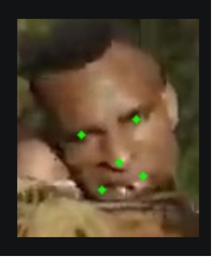
\includegraphics[width=\textwidth]{figures/contoh-fitur-geometris}
\caption{Empat titik fitur geometris}
\end{subfigure}
\hfill
\begin{subfigure}[b]{0.3\textwidth}
\centering
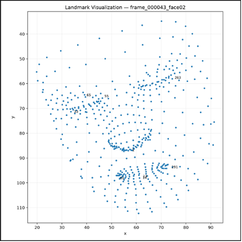
\includegraphics[width=\textwidth]{figures/contoh-visualisasi-titik-fitur}
\caption{Visualisasi \textit{mesh} 468-titik}
\end{subfigure}
\caption[Tiga tahap representasi untuk satu potongan wajah yang sama]{Tiga tahap representasi untuk satu potongan wajah yang sama: (a) hasil pemotongan langsung dari pendeteksi SCRFD, (b) empat titik fitur geometris MediaPipe (jarak alis, sudut bibir, bukaan mulut, jarak antar-mata), dan (c) \textit{mesh} 468-titik penuh milik MediaPipe yang dipakai untuk menurunkan titik-titik pada (b). Panel (b) dan (c) adalah fitur geometris dari \textit{pipeline} lama (lihat juga Bab~\ref{chap:literature-review}) dan bukan masukan bagi tiga eksperimen FER pada Bab~\ref{chap:results}; disertakan di sini semata untuk memperjelas apa yang dimaksud ``titik-fitur'' bagi pembaca yang tidak terbiasa dengan istilah \textit{computer vision}.}
\label{fig:tiga-tahap-wajah}
\end{figure}

\subsection{HSEmotion: Inferensi dengan Model Terlatih}

Berkas ekspor ONNX milik HSEmotion (\texttt{enet\_b0\_8\_best\_vgaf}) dijalankan persis seperti yang dipublikasikan: bobotnya tidak diubah di mana pun dalam proyek ini, dan keluaran \textit{softmax}-nya atas kosakata delapan-kelas yang sudah tetap (Marah, Jijik, Takut, Senang, Netral, Sedih, Terkejut, dan Merendahkan, \textit{Contempt}) diambil langsung sebagai prediksi. Kelas \textit{Contempt} tidak punya padanan pada label manusia; pada 227 potongan, HSEmotion tidak sekali pun memprediksi \textit{Contempt}, sehingga kelas ini tidak memengaruhi hasil apa pun dalam tesis ini. Ini adalah satu-satunya konfigurasi yang dipakai pada EXP-005 maupun EXP-006; kedua eksperimen hanya berbeda pada apakah CLAHE diterapkan pada potongan wajah sebelum tahap ini dijalankan.

\subsection{Konfigurasi CLAHE (RQ2)}
\label{sec:clahe-config}

Varian CLAHE pada EXP-006 berada di \texttt{notebooks/\allowbreak preprocessing\_experiment.ipynb} dan secara eksplisit bukan bagian dari \textit{pipeline} produksi (\texttt{src/\allowbreak fer\_dataset/\allowbreak pipeline/\allowbreak emotion\_classifier.py} tidak menerapkan praproses semacam ini). Transformasi ini hanya bekerja pada kanal-L ruang warna LAB, dengan batas klip yang menyesuaikan estimasi kecerahan berbobot tiap potongan, antara batas bawah 1,5 dan batas atas 3,5, pada rentang kecerahan masukan 60--220, diterapkan dengan kisi ubin (\textit{tile}) $8\times8$. Setiap potongan yang sudah disesuaikan dengan CLAHE kemudian diklasifikasi ulang dengan model HSEmotion beku yang sama seperti pada EXP-005, dan hasilnya dibandingkan terhadap prediksi pada potongan asli (tanpa modifikasi) dari eksperimen yang sama, pada 227 potongan yang sama, sehingga perbandingan sebelum/sesudah ini bersifat model-sama, sampel-sama, hanya satu varian praproses yang berubah. Ini adalah satu kali eksekusi saja, tanpa pengulangan, dan EXP-006 sendiri tidak menghitung selang kepercayaan maupun uji signifikansi. Selang kepercayaan dan uji McNemar untuk perbandingan ini kemudian dihitung pada subset 135 potongan oleh EXP-011, dari prediksi EXP-006 yang sudah tersimpan tanpa inferensi ulang (\S\ref{sec:fairness-methods}).

\subsection{\textit{Embedding} ArcFace dan Klasifier Regresi Logistik (RQ3)}
\label{sec:arcface-config}

\textit{Embedding} ArcFace dihasilkan dengan menjalankan ulang deteksi dan penyelarasan (\textit{alignment}) wajah pada setiap gambar potongan 227-potongan yang sudah ada (bukan pada \textit{frame} video asli), melalui submodel \texttt{buffalo\_l/w600k\_r50} milik InsightFace, menghasilkan vektor 512-dimensi yang sudah dinormalisasi-L2 untuk setiap potongan yang berhasil diselaraskan. Langkah deteksi ulang inilah sumber dari hitungan 178-dari-227 keberhasilan penyelarasan (\S\ref{sec:dataset-overview}), dan tempat terjadinya 6 dari pengecualian akhir populasi 135 potongan. Bobot ArcFace dibekukan sepenuhnya: ArcFace hanya menyumbang representasi yang tetap, tidak ada yang disesuaikan (\textit{fine-tuned}) pada data proyek ini.

Klasifier yang dilatih di atas \textit{embedding} ini adalah Regresi Logistik multinomial, teregularisasi-L2, berbobot-kelas, dipilih dan divalidasi dengan validasi silang \texttt{StratifiedGroupKFold} lima-lipatan (\textit{seed} 42), dengan potongan-potongan dikelompokkan ke dalam blok temporal 3-\textit{frame} sebelum dibagi ke lipatan. Pengelompokan ini ada karena tidak tersedia kolom identitas subjek pada dataset ini (\S\ref{sec:leakage}); pengelompokan berdasarkan kedekatan waktu adalah pengganti heuristik, bukan jaminan terverifikasi bahwa individu yang sama tidak pernah muncul di dua lipatan berbeda. Tidak ada partisi uji terpisah yang disisihkan di luar lipatan validasi silang. Angka akurasi dan pola kesalahan yang dilaporkan pada Bab~\ref{chap:results} \S\ref{sec:rq3-results} adalah estimasi hasil validasi silang atas seluruh populasi 135 potongan, bukan dari satu pembagian latih/uji tunggal.

\subsection{Metrik Evaluasi}
\label{sec:metrics}

Tiga prosedur statistik dipakai, masing-masing untuk tujuan tertentu, dan tidak satu pun bisa saling menggantikan. Uji McNemar \citep{mcnemar1947note} (EXP-007, RQ3) membandingkan pasangan hasil benar/salah dari dua klasifier pada 135 potongan yang sama, sebuah pemakaian yang direkomendasikan \citet{dietterich1998approximate} untuk membandingkan dua klasifier yang masing-masing hanya dijalankan sekali karena tingkat galat tipe I-nya rendah, dan menguji apakah ketidaksepakatan di antara keduanya simetris; uji ini menjawab ``apakah ada perbedaan yang terdeteksi,'' bukan ``apakah kedua klasifier setara''. Perbedaan ini terus ditegaskan pada Bab~\ref{chap:results} mengingat sampel ini hanya punya 46 pasangan yang tidak sepakat. \textit{Bootstrap} yang sadar-kelompok (2.000 pengambilan ulang sampel, mengambil ulang berdasarkan 16 kelompok temporal, bukan per potongan individu) menghasilkan selang kepercayaan 95\% untuk akurasi tiap klasifier, menghormati ketidak-bebasan data yang sama yang melandasi validasi silang berkelompok di atas. Uji eksak Fisher (EXP-005/007) menguji apakah kelompok proksi warna kulit dan kebenaran klasifikasi berasosiasi secara statistik pada sampel ini; hasil yang signifikan dari uji ini adalah bukti adanya asosiasi pada sampel khusus dan tidak acak ini, bukan bukti bahwa variabel proksi tersebut menyebabkan hasil klasifikasi.

\subsection{Evaluasi Kesenjangan Antar-Kelompok (EXP-010 dan EXP-011)}
\label{sec:fairness-methods}

Ketiga RQ dijawab pada populasi yang sama, yaitu subset 135 potongan lima-kelas (\S\ref{sec:dataset-overview}). Kedua eksperimen ini adalah analisis ulang atas prediksi yang sudah tersimpan: tidak ada model yang dilatih atau dijalankan ulang, dan tidak ada label, dataset, atau berkas prediksi yang diubah. EXP-010 membaca prediksi HSEmotion dan ArcFace + LR dari EXP-007; EXP-011 membaca prediksi HSEmotion pada potongan asli dan potongan CLAHE dari EXP-006. Keduanya dapat direproduksi dengan \texttt{tools/\allowbreak analyze\_fairness\_135.py} dan \texttt{tools/\allowbreak analyze\_clahe\_fairness\_135.py}, dan keluarannya terbukti identik pada setiap jalan.

\textbf{Pengelompokan.} Pada EXP-007/008, kelompok kecerahan hanya tersedia untuk 78 dari 135 potongan, karena diambil dari berkas fitur titik-fitur wajah yang hanya mencakup 85 potongan. EXP-010 menjalankan fungsi yang sama (\texttt{\_compute\_skin\_tone}) pada potongan \textbf{asli} untuk seluruh 135 potongan. Hasilnya mereproduksi ke-78 kelompok yang sudah ada tanpa perbedaan (78/78) dan menghasilkan Gelap 89 dan Gelap-Sedang 46; tidak ada potongan Gelap-Terang atau Terang. Hasil dilaporkan dengan pengelompokan 135 potongan sebagai analisis utama dan pengelompokan 78 potongan sebagai pemeriksaan stabilitas. Pada EXP-011, kelompok yang sama dipakai untuk kedua kondisi, sehingga CLAHE tidak memindahkan potongan antar-kelompok; kolom kelompok pada berkas EXP-006 juga cocok dengan kelompok ini pada 135/135 potongan.

\textbf{Pemetaan kelas.} Label HSEmotion dipetakan ke penamaan tesis ini (\textit{Anger}$\to$Marah, \textit{Happiness}$\to$Senang, \textit{Sadness}$\to$Sedih), sama dengan pemetaan pada \texttt{tools/\allowbreak evaluate\_arcface\_vs\_hsemotion.py}. Prediksi Marah dihitung sebagai salah karena berada di luar lima kelas evaluasi. Berkas EXP-006 menyimpan label yang sudah dipetakan, sedangkan EXP-007 menyimpan nama asli keluaran model; perbandingan literal hanya cocok pada 88 dari 135 potongan, tetapi setelah pemetaan yang sama, prediksi potongan asli EXP-006 identik dengan prediksi HSEmotion EXP-007 pada 135/135 potongan. Perbedaan ini hanya soal penamaan, bukan perbedaan data.

\textbf{Metrik.}
\begin{itemize}
  \item \textit{Akurasi}: proporsi potongan yang prediksinya sama dengan kebenaran lapangan.
  \item \textit{F1 makro}: rata-rata F1 tiap kelas. Untuk keseluruhan, dirata-ratakan atas lima kelas; untuk tiap kelompok, atas kelas yang ada pada kelompok tersebut.
  \item \textit{Kesenjangan}: akurasi Gelap dikurangi akurasi Gelap-Sedang.
  \item \textit{Akurasi kelompok terburuk}: akurasi terendah di antara kedua kelompok, ukuran yang lazim dipakai untuk menilai kinerja model pada kelompok yang paling dirugikan \citep{sagawa2020dro}.
  \item \textit{Recall} per kelas di dalam kelompok, hanya untuk Netral dan Senang, karena kelas lain terlalu kecil pada kelompok Gelap-Sedang.
\end{itemize}

\textbf{Perbandingan.} EXP-010 membandingkan HSEmotion dan ArcFace + LR, termasuk selisih kesenjangan kedua model (kesenjangan HSEmotion dikurangi kesenjangan ArcFace + LR). EXP-011 membandingkan HSEmotion pada potongan asli dan potongan CLAHE, dengan perubahan dihitung sebagai CLAHE dikurangi asli untuk akurasi, akurasi per kelompok, dan kesenjangan.

\textbf{Uji dan selang kepercayaan.} Uji McNemar eksak (uji binomial atas pasangan yang tidak sepakat) dijalankan untuk seluruh potongan dan untuk tiap kelompok. Selang kepercayaan 95\% dihitung dengan \textit{bootstrap} berkelompok yang sama dengan EXP-007: 16 blok waktu (indeks \textit{frame} dibagi 3) diambil ulang dengan pengembalian, 2.000 kali, dan batas 2,5 serta 97,5 persentil diambil sebagai selang. Gagasan mengambil ulang blok observasi yang berurutan, bukan observasi tunggal, untuk data yang saling bergantung berasal dari \textit{block bootstrap} \citep{kunsch1989jackknife}. Varian yang dipakai di sini lebih sederhana: blok tetap yang tidak tumpang-tindih dan panjangnya ditentukan secara heuristik (3 \textit{frame}), bukan blok bergerak dengan panjang yang dipilih secara teoretis. Pengelompokan ini hanya mengatasi ketergantungan antar-potongan dari \textit{frame} yang berdekatan; pengelompokan ini tidak mengendalikan kemunculan ulang orang yang sama di bagian film yang berjauhan (\S\ref{sec:leakage}). Setiap selang memakai pembangkit acak baru dengan \textit{seed} 42. Untuk ukuran yang membandingkan dua kelompok atau dua kondisi (kesenjangan, selisih kesenjangan, perubahan akurasi), kedua sisi dihitung pada sampel \textit{bootstrap} yang sama, sehingga perbandingannya berpasangan. F1 makro dilaporkan tanpa selang kepercayaan.

\textbf{Batasan analisis.} Uji McNemar per kelompok dan seluruh perbandingan antar-kelompok tidak dikoreksi untuk perbandingan berganda dan diperlakukan sebagai eksploratif. Kedua eksperimen bersifat retrospektif: prediksi yang dianalisis sudah ada sebelum RQ dirumuskan. HSEmotion dipakai apa adanya, sedangkan prediksi ArcFace + LR berasal dari validasi silang berkelompok (\S\ref{sec:arcface-config}), sehingga kedua model tidak dievaluasi dengan protokol yang sama. Kelompok Gelap-Sedang hanya berisi 46 potongan, sehingga daya uji per kelompok rendah; hasil yang tidak signifikan tidak dibaca sebagai bukti tidak adanya pengaruh. \textit{Bootstrap} blok waktu hanya sebagian mengatasi kemunculan orang yang sama pada beberapa potongan (\S\ref{sec:leakage}).

\section{Titik-Fitur Wajah: Jalur Pendukung yang Masih Berjalan}
\label{sec:methodology-landmarks}

\subsection{Papuan V2}
\label{sec:papuan-v2}

Papuan V2 adalah ekstraksi kedua yang independen dari film sumber yang sama, dengan jalan pengambilan sampel yang berbeda (\texttt{max\_frames=250}, 2,0 fps), menghasilkan 645 potongan wajah dengan cabang olahan-CLAHE paralel, dan tidak berbagi satu pun potongan dengan populasi 227/135 potongan yang dipakai untuk RQ1 sampai RQ3. Subset uji coba berjumlah 150 gambar diambil untuk uji coba anotasi, dan alur kerja anotasi manusia disiapkan memakai dua instansi server Label Studio yang terisolasi: satu untuk anotator utama yang mengerjakan seluruh 150 gambar uji coba, satu lagi untuk anotator kedua yang mengerjakan subset tumpang-tindih 75 gambar yang dimaksudkan untuk mendukung pengukuran kesepakatan antar-anotator begitu keduanya selesai. Tidak satu pun yang selesai: antrean tugas anotator tumpang-tindih menunjukkan nol dari 75 tugas terkumpul pada status terakhir yang tercatat, dan klaim penyelesaian penuh oleh anotator utama belum diverifikasi ulang secara independen terhadap berkas ekspor mentahnya untuk revisi ini (\texttt{research-audit/DATA\_DISCREPANCIES.md} D-1). Secara terpisah, HSEmotion dan klasifier berbasis ArcFace sama-sama dijalankan terhadap 150 gambar uji coba ini, menghasilkan prediksi tanpa ada label manusia yang tersedia untuk dibandingkan.

\subsection{Dari Label Emosi ke Titik-Fitur, dan Posisi Uji Coba Ini Sekarang}

Di tengah perjalanan proyek ini, target anotasi untuk uji coba Papuan V2 diubah, atas arahan dosen pembimbing, dari label emosi menjadi titik-fitur wajah. Perubahan ini terbatas pada target anotasi uji coba ini saja, bukan perubahan arah penelitian tesis secara keseluruhan, yang tetap FER (\texttt{RESEARCH\_DECISIONS.md}, Keputusan 2). Konvensi yang dipakai adalah 68 titik mengikuti ibug-300W, dengan koordinat awal dibuat otomatis oleh submodel \texttt{landmark\_3d\_68} milik InsightFace dan dimuat ke instansi CVAT lokal untuk diperiksa. Uji coba 24-gambar diisi dengan cara ini, dan skema penamaan titik milik proyek ini sendiri ditulis ulang dari pengenal generik (\texttt{pt0} hingga \texttt{pt67}) menjadi nama anatomis yang deskriptif, perubahan yang sudah diverifikasi tidak menggeser koordinat sama sekali.

\begin{figure}[htbp]
\centering
\begin{subfigure}[b]{0.32\textwidth}
\centering
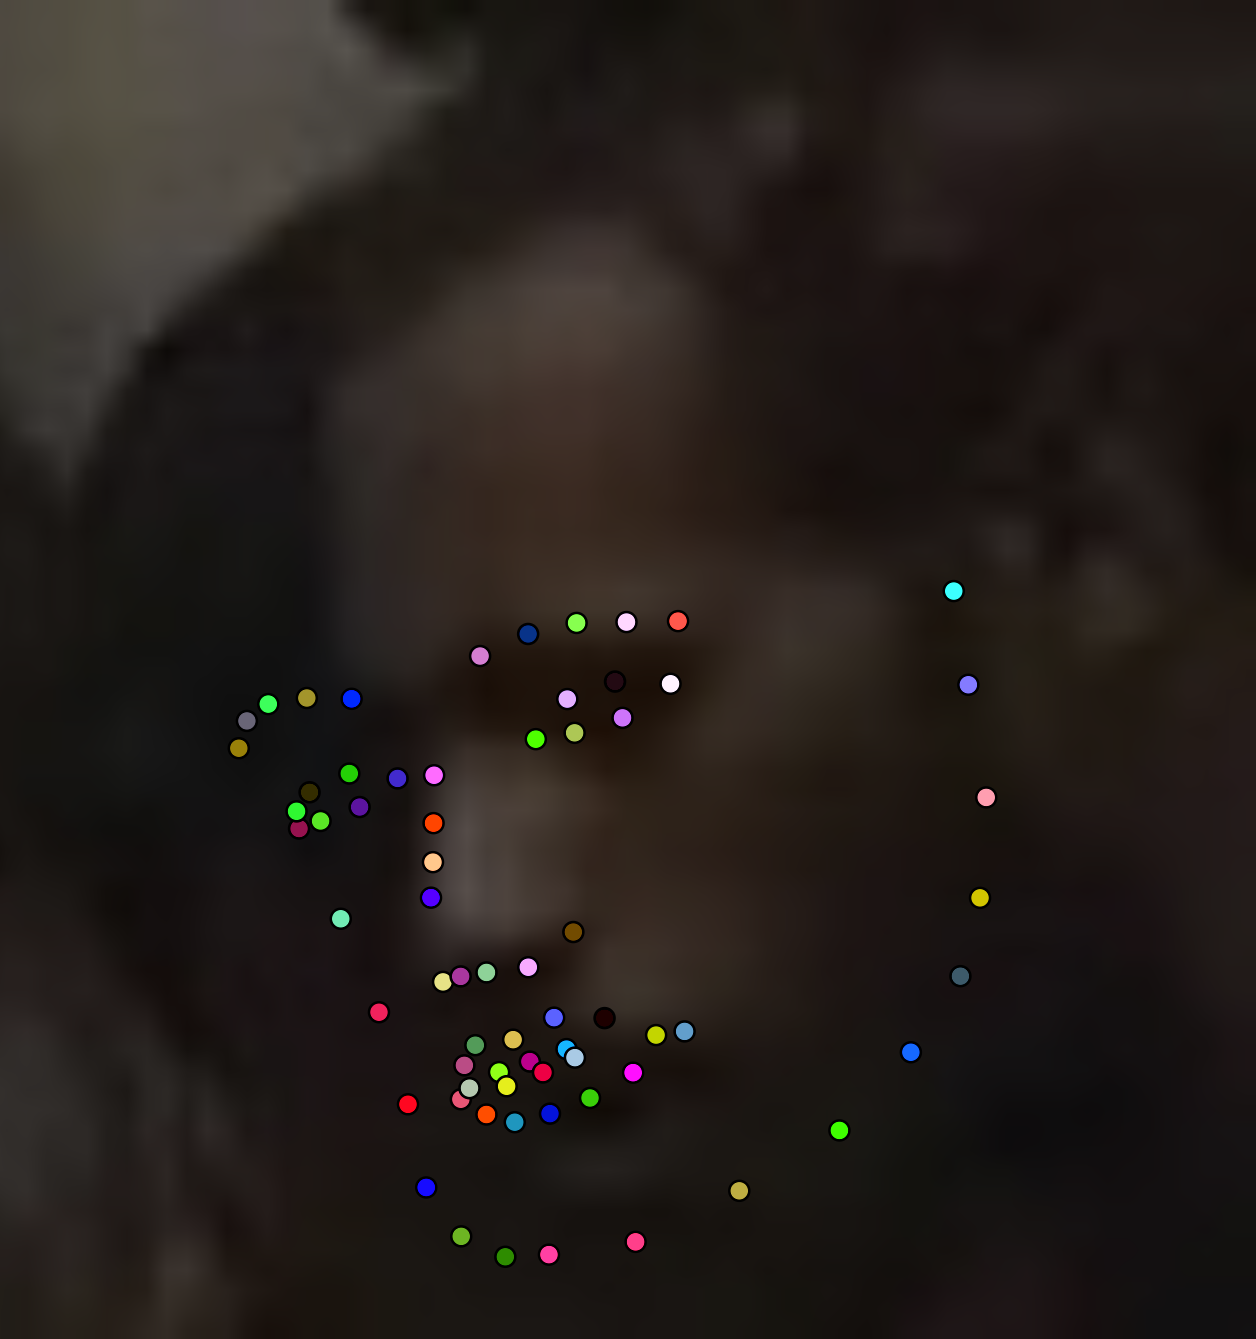
\includegraphics[width=\textwidth]{figures/contoh-anotasi-cvat-68-titik}
\caption{68 titik usulan otomatis}
\end{subfigure}
\hfill
\begin{subfigure}[b]{0.3\textwidth}
\centering
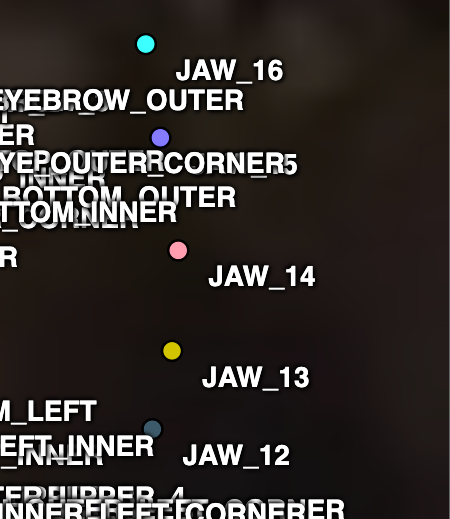
\includegraphics[width=\textwidth]{figures/contoh-label-anatomis-kanvas-cvat}
\caption{Label anatomis pada kanvas}
\end{subfigure}
\hfill
\begin{subfigure}[b]{0.3\textwidth}
\centering
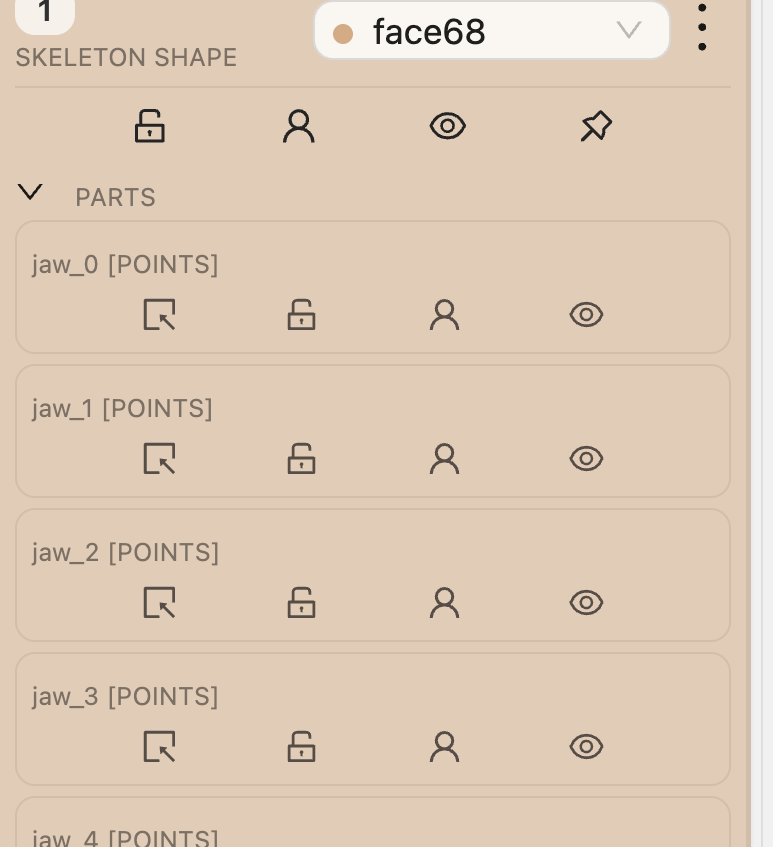
\includegraphics[width=\textwidth]{figures/contoh-skema-penamaan-cvat}
\caption{Panel \textit{Parts} CVAT}
\end{subfigure}
\caption[Tangkapan layar uji coba CVAT 24-gambar]{Tangkapan layar instansi CVAT lokal pada uji coba 24-gambar, potongan wajah \texttt{frame\_000009\_face04}: (a) 68 titik usulan otomatis dari submodel \texttt{landmark\_3d\_68} milik InsightFace, sebelum pemeriksaan manusia; (b) label anatomis (mis.\ \texttt{JAW\_16}, \texttt{JAW\_14}) tampil langsung pada kanvas, menggantikan pengenal generik \texttt{pt0}--\texttt{pt67}; (c) panel \textit{Parts} CVAT yang sama menunjukkan skema penamaan (\texttt{jaw\_0}, \texttt{jaw\_1}, dst.) untuk \textit{skeleton shape} \texttt{face68}. Titik-titik ini adalah usulan otomatis yang belum diperiksa; tidak ada koreksi manusia yang terekam pada tangkapan layar ini.}
\label{fig:cvat-pilot-68-titik}
\end{figure}

\textbf{Pembaruan sejak revisi sebelumnya: pemeriksaan manusia dan uji coba pelatihan awal sudah dilakukan, tetapi hasilnya tetap bersifat awal (\textit{preliminary}) dan tidak menunjukkan hasil yang meyakinkan.} Pemeriksaan manusia sudah diselesaikan untuk 64 gambar Original: 24 gambar dari uji coba awal (CVAT Task 1) dan 40 gambar tambahan dari uji coba kalibrasi (CVAT Task 3), keduanya diperiksa oleh satu peninjau yang sama -- belum ada peninjau kedua atau protokol kesepakatan antar-peninjau untuk titik-fitur, keterbatasan yang sejajar dengan yang sudah dinyatakan untuk populasi 227/135 potongan pada \S\ref{sec:dataset-overview}. Dari 64 gambar yang sudah diperiksa ini, satu pembagian \textit{train}/\textit{validation}/\textit{test} (45/11/8 gambar) dibuat dengan benih tetap (\texttt{seed=400}), dikelompokkan berdasarkan kedekatan nomor \textit{frame} karena tidak ada kolom identitas subjek yang tersedia di repositori ini -- keterbatasan yang sama persis dengan \S\ref{sec:leakage}, bukan jaminan bebas-kebocoran yang terverifikasi.

Dua model dasar dilatih dan dievaluasi pada pembagian ini, keduanya pada potongan Original saja: (1) model rerata-bentuk (\textit{mean-shape}) yang sepenuhnya mengabaikan isi piksel gambar, sebagai batas bawah pembanding; dan (2) regresi Ridge (\texttt{sklearn.linear\_model.Ridge}) pada fitur piksel \textit{grayscale} $32\times32$ yang diubah ukurannya dan diratakan (1.024 fitur), meregresi ke-68 titik sekaligus. \textbf{Regresi Ridge belum menunjukkan perbaikan yang berarti dibandingkan model rerata-bentuk pada 8 gambar uji yang disisihkan} -- Gambar~\ref{fig:ridge-vs-meanshape} menunjukkan galat piksel yang hampir identik di antara keduanya pada hampir setiap gambar uji, bukan hanya pada rata-ratanya. Model Ridge yang sama (tidak dilatih ulang) juga dievaluasi pada versi CLAHE dari gambar uji yang sama, memakai koordinat target yang tidak diubah -- sah dilakukan karena CLAHE pada proyek ini sudah diverifikasi secara terpisah tidak mengubah geometri gambar (lihat Gambar~\ref{fig:titik-clahe-original}). Hasilnya juga hampir identik dengan versi Original, yang konsisten dengan model ini belum benar-benar memanfaatkan isi piksel secara berarti -- \textbf{ini bukan bukti bahwa model titik-fitur yang sungguh-sungguh belajar dari piksel akan menunjukkan ketahanan yang sama terhadap CLAHE}, hanya bahwa model saat ini belum cukup sensitif terhadap piksel untuk diuji pada pertanyaan itu.

\begin{figure}[htbp]
\centering
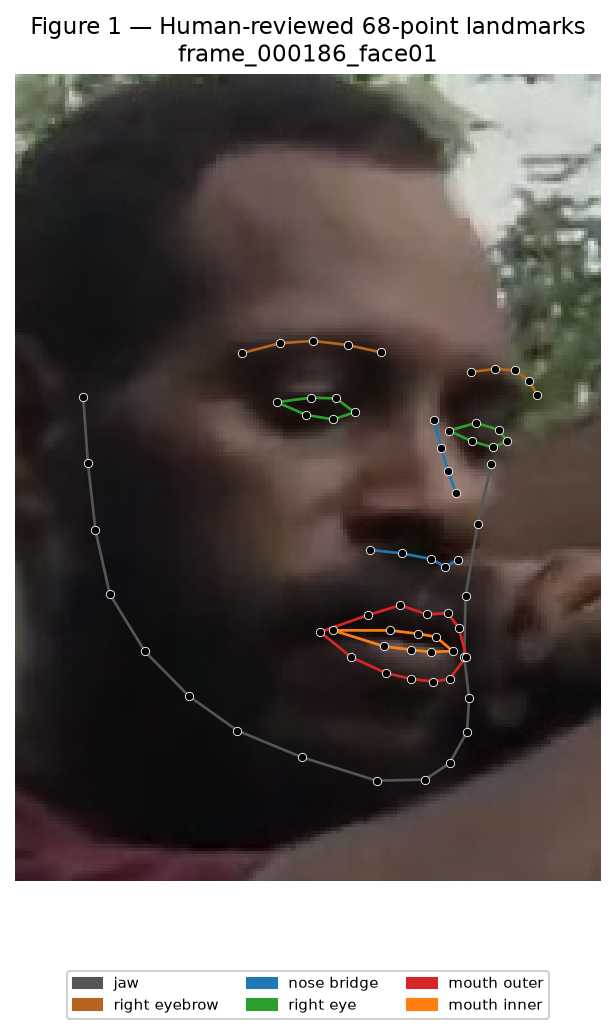
\includegraphics[width=0.7\textwidth]{figures/contoh-titik-fitur-diperiksa-manusia}
\caption[Contoh titik-fitur yang sudah diperiksa manusia]{Satu gambar dengan 68 titik-fitur yang sudah diperiksa manusia, diberi warna menurut wilayah wajah (rahang, alis, mata, hidung, mulut).}
\label{fig:titik-fitur-diperiksa}
\end{figure}

\begin{figure}[htbp]
\centering
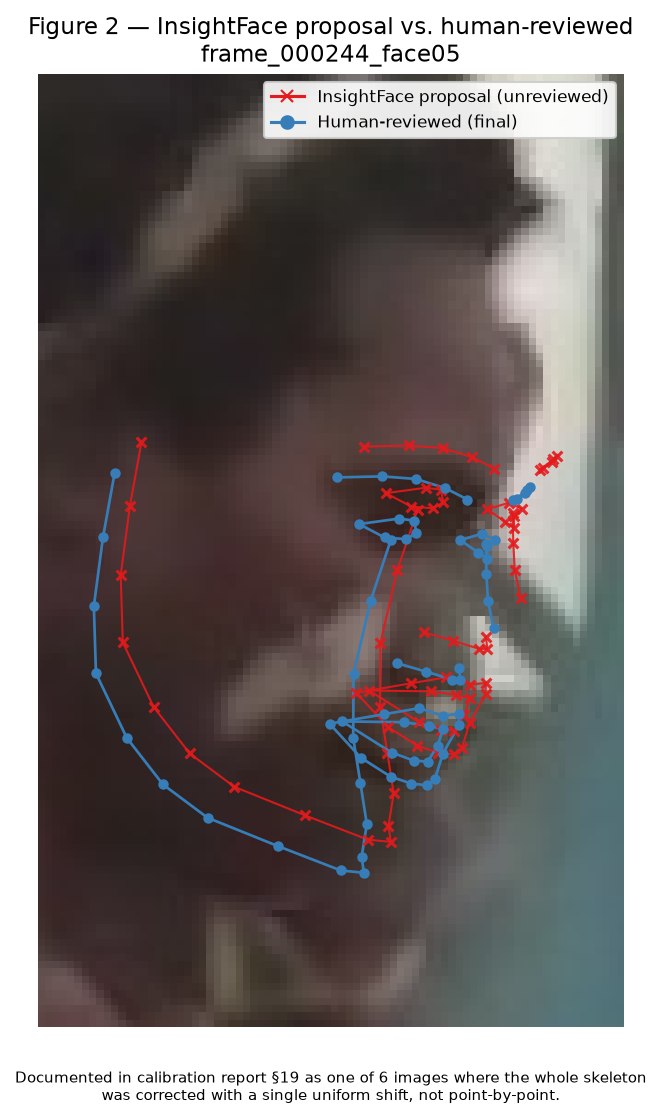
\includegraphics[width=0.6\textwidth]{figures/perbandingan-usulan-vs-diperiksa}
\caption[Usulan otomatis dibandingkan hasil pemeriksaan manusia]{Usulan otomatis InsightFace (merah, tanda ×) dibandingkan hasil akhir setelah pemeriksaan manusia (biru, titik) pada gambar yang sama -- satu dari beberapa gambar yang dikoreksi dengan menggeser seluruh \textit{skeleton} sekaligus, bukan titik demi titik, sebagaimana didokumentasikan dalam catatan uji coba kalibrasi proyek ini.}
\label{fig:usulan-vs-diperiksa}
\end{figure}

\begin{figure}[htbp]
\centering
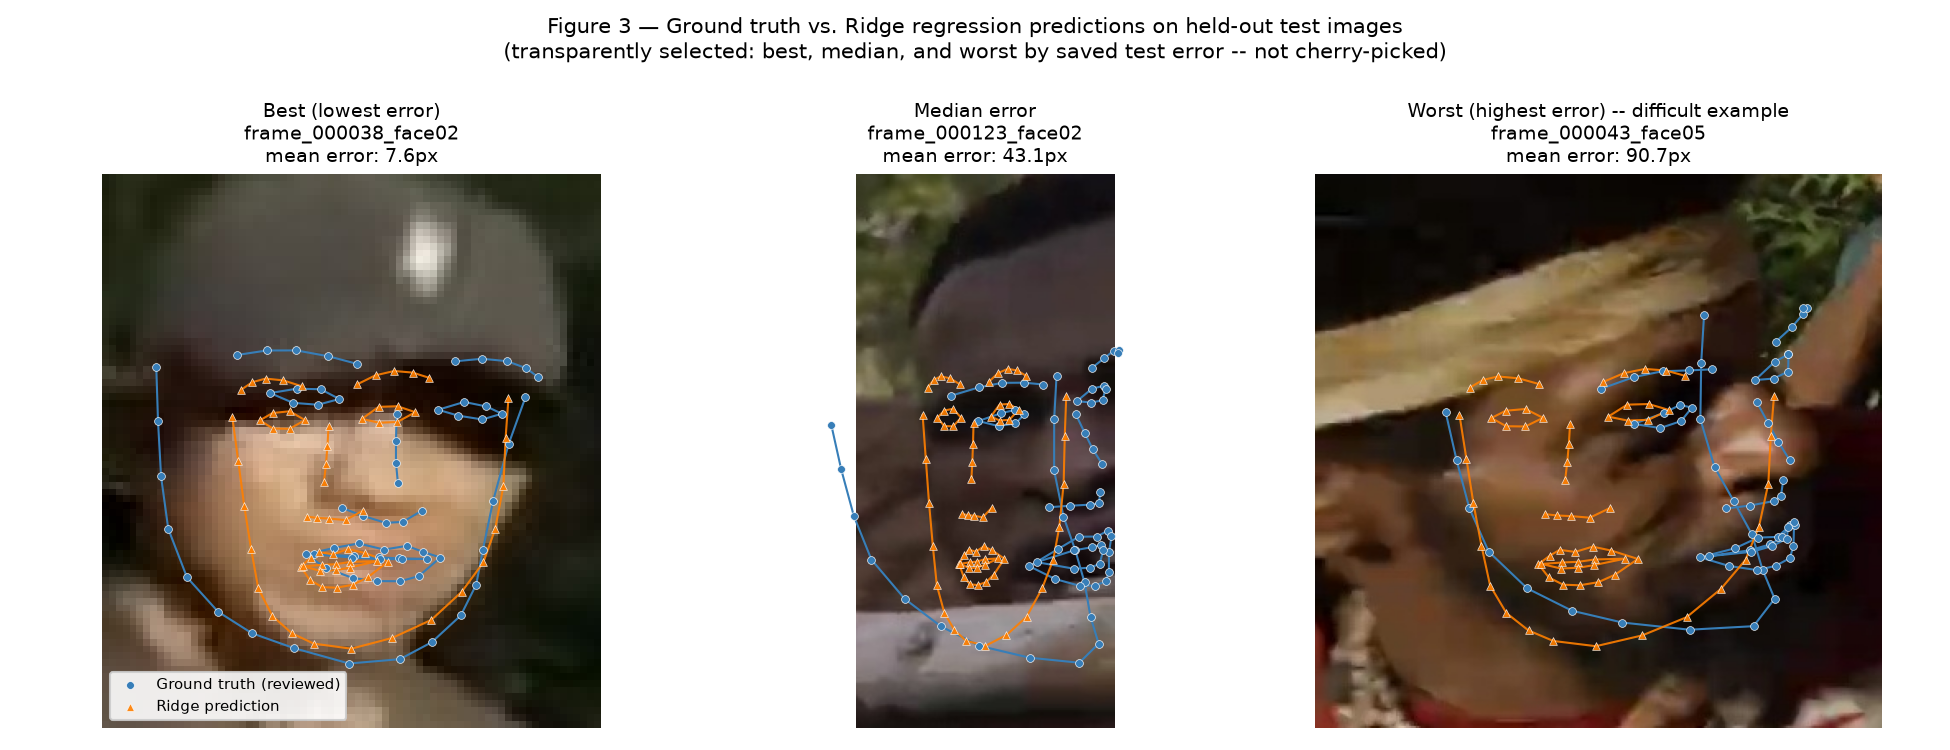
\includegraphics[width=0.85\textwidth]{figures/kebenaran-vs-prediksi-ridge}
\caption[Kebenaran lapangan dibandingkan prediksi Ridge pada gambar uji]{Kebenaran lapangan (biru) dibandingkan prediksi regresi Ridge (oranye) pada tiga gambar uji yang dipilih secara transparan -- gambar dengan galat terendah, median, dan tertinggi dari seluruh 8 gambar uji -- bukan dipilih karena hasilnya terlihat baik.}
\label{fig:ridge-vs-meanshape}
\end{figure}

\begin{figure}[htbp]
\centering
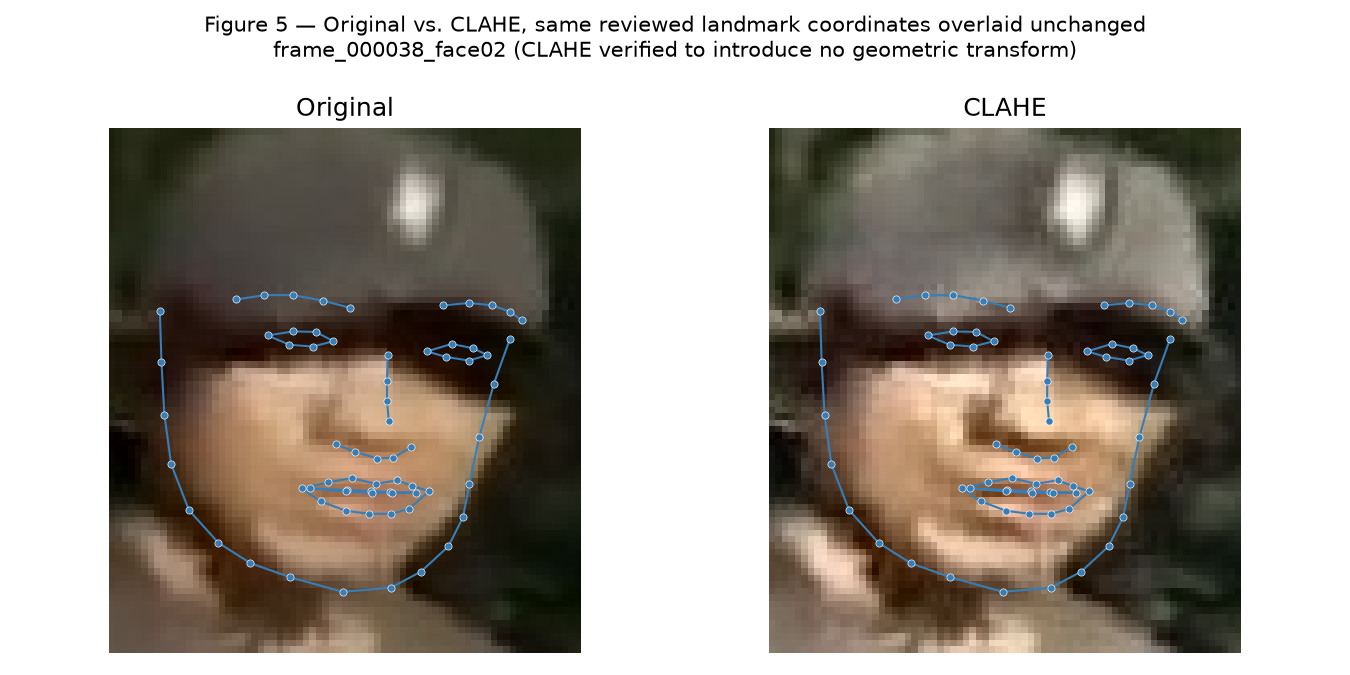
\includegraphics[width=0.75\textwidth]{figures/titik-fitur-original-vs-clahe}
\caption[Titik-fitur yang sama pada gambar Original dan CLAHE]{Koordinat titik-fitur hasil pemeriksaan manusia yang identik, ditumpangkan tanpa perubahan pada versi Original (kiri) dan CLAHE (kanan) dari potongan wajah yang sama -- mengonfirmasi secara visual bahwa transformasi CLAHE pada proyek ini tidak mengubah geometri gambar.}
\label{fig:titik-clahe-original}
\end{figure}

Yang masih belum ada, dinyatakan secara eksplisit agar tidak tersirat lebih dari yang sebenarnya: belum ada peninjau kedua atau statistik kesepakatan antar-peninjau untuk titik-fitur; cakupan pemeriksaan baru 64 dari 645 gambar yang tersedia ($<$10\%); belum ada bukti bahwa pendekatan berbasis piksel apa pun benar-benar mengungguli \textit{mean-shape} pada data sebesar ini; dan tidak ada klaim ketahanan umum terhadap CLAHE, soal keadilan (\textit{fairness}), maupun generalisasi di luar sampel kecil ini. Rincian lengkap metodologi pelatihan, pembagian data, dan hasil per-gambar didokumentasikan di luar naskah tesis ini pada \texttt{docs/reports/PAPUAN\_V2\_ANNOTATION\_CALIBRATION\_PLAN.md} (artefak repositori, bukan lampiran tesis formal). Masing-masing dari keterbatasan ini adalah kerja lanjutan, didaftar beserta bukti yang diperlukan untuk menyatakannya selesai, pada Bab~\ref{chap:conclusion} \S\ref{sec:future-work}. Tidak ada apa pun dalam tesis ini yang mengklaim, menyiratkan, atau bergantung pada uji coba ini sudah terbukti berguna atau dapat diandalkan sebagai model titik-fitur, dan tidak ada satu pun hasil pada Bab~\ref{chap:results} yang bersyarat pada hal itu.

\section{Identitas Subjek, Kebocoran Data, dan Batas Kemampuan Pengelompokan}
\label{sec:leakage}

Tidak ada kolom pada kedua dataset yang menandai potongan mana saja yang menunjukkan orang yang sama. Pengelompokan temporal 3-\textit{frame} yang dipakai untuk validasi silang EXP-007 (\S\ref{sec:arcface-config}) berasumsi bahwa \textit{frame} yang berdekatan waktu lebih mungkin menunjukkan subjek yang sama dalam pose yang nyaris identik dibanding \textit{frame} yang berjauhan. Ini adalah heuristik yang masuk akal untuk rekaman dokumenter satu kamera, tetapi bukan jaminan yang terverifikasi. Seorang subjek yang keluar lalu muncul kembali ke adegan di bagian film yang lebih belakangan akan terpecah ke kelompok yang berbeda oleh skema ini, dan tidak ada apa pun dalam \textit{pipeline} saat ini yang akan menangkap kejadian tersebut. Hal ini membatasi seberapa kuat estimasi validasi silang pada \S\ref{sec:rq3-results} bisa dibaca sebagai bebas-dari-pengaruh-subjek-yang-sama, dan hal ini dinyatakan ulang pada bagian Bab~\ref{chap:results} di mana hal ini relevan dengan angka tertentu, bukan hanya di sini.
